\chapter{Density Functions}

\subsubsection{Multivariate Gaussian}

\begin{equation}
    p(\mathbf{x}) = \frac{1}{\sqrt{(2\pi)^n |\boldsymbol{\Sigma}|}} \exp\left(-\frac{1}{2} (\mathbf{x} - \boldsymbol{\mu})^T \boldsymbol{\Sigma}^{-1} (\mathbf{x} - \boldsymbol{\mu})\right)
    \label{eq:mvn}
\end{equation}

\subsubsection{Log Multivariate Gaussian}

\begin{equation}
    \log p(\mathbf{x}) = -\frac{n}{2} \log(2\pi) - \frac{1}{2} \log |\boldsymbol{\Sigma}| - \frac{1}{2} (\mathbf{x} - \boldsymbol{\mu})^T \boldsymbol{\Sigma}^{-1} (\mathbf{x} - \boldsymbol{\mu})
    \label{eq:log_mvn}
\end{equation}


\chapter{Additional Experiment Results}

\subsubsection{Spirals Repeat}
\label{sec:app_spirals}

\begin{figure}[H]
    \centering
    \makebox[\textwidth][c]{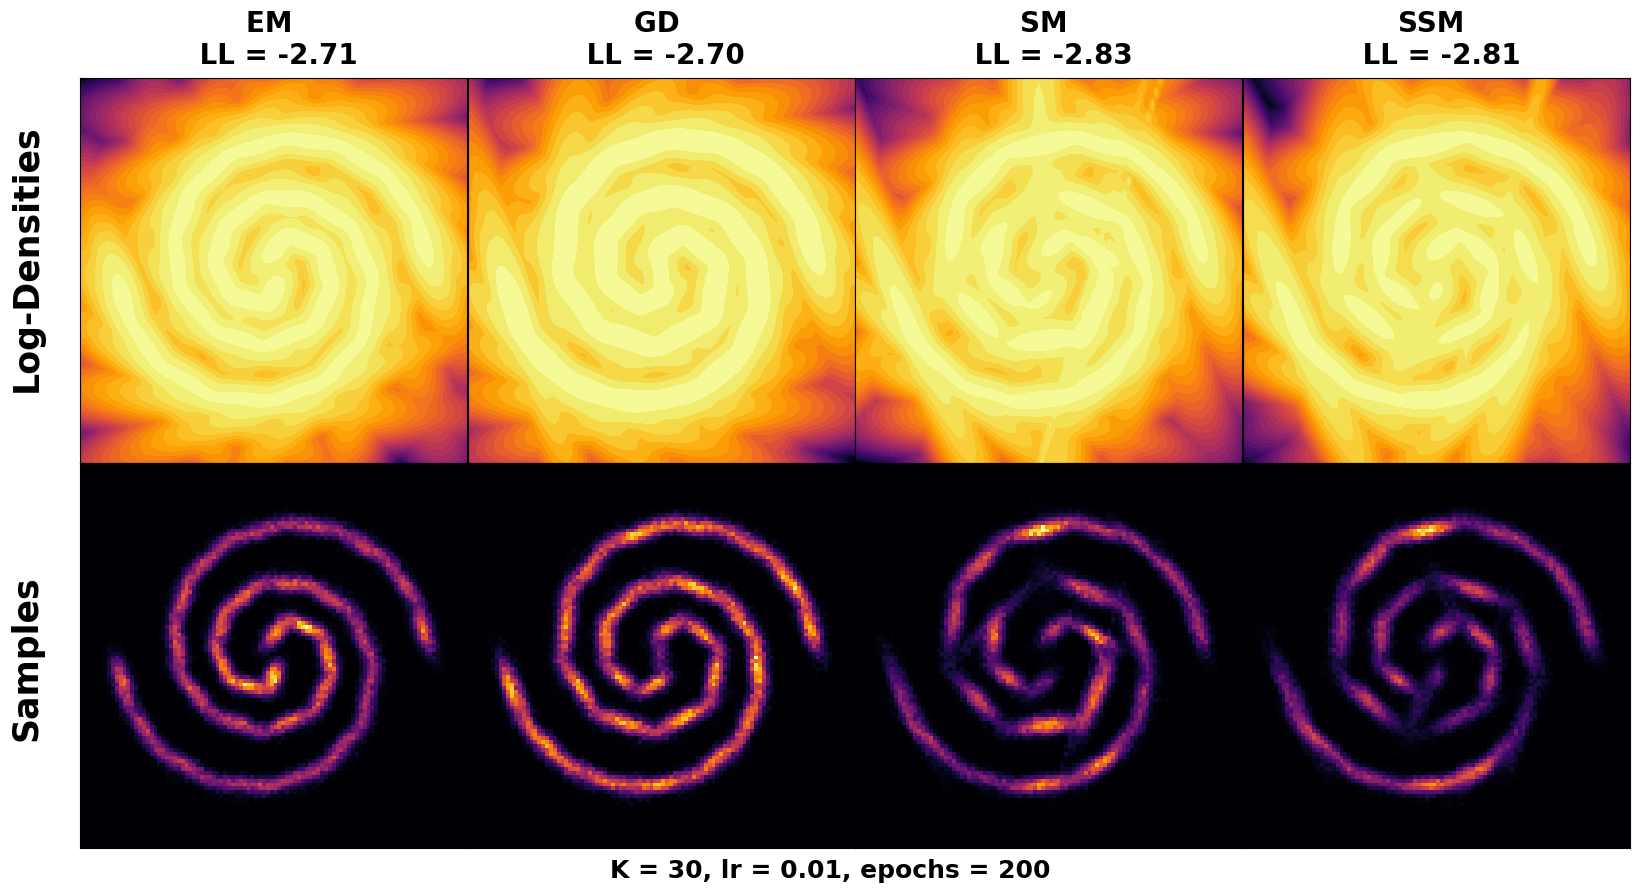
\includegraphics[width=0.6\textwidth]{figures/spirals/30_kmeans.png}}
    \makebox[\textwidth][c]{\hspace{-0.4cm} 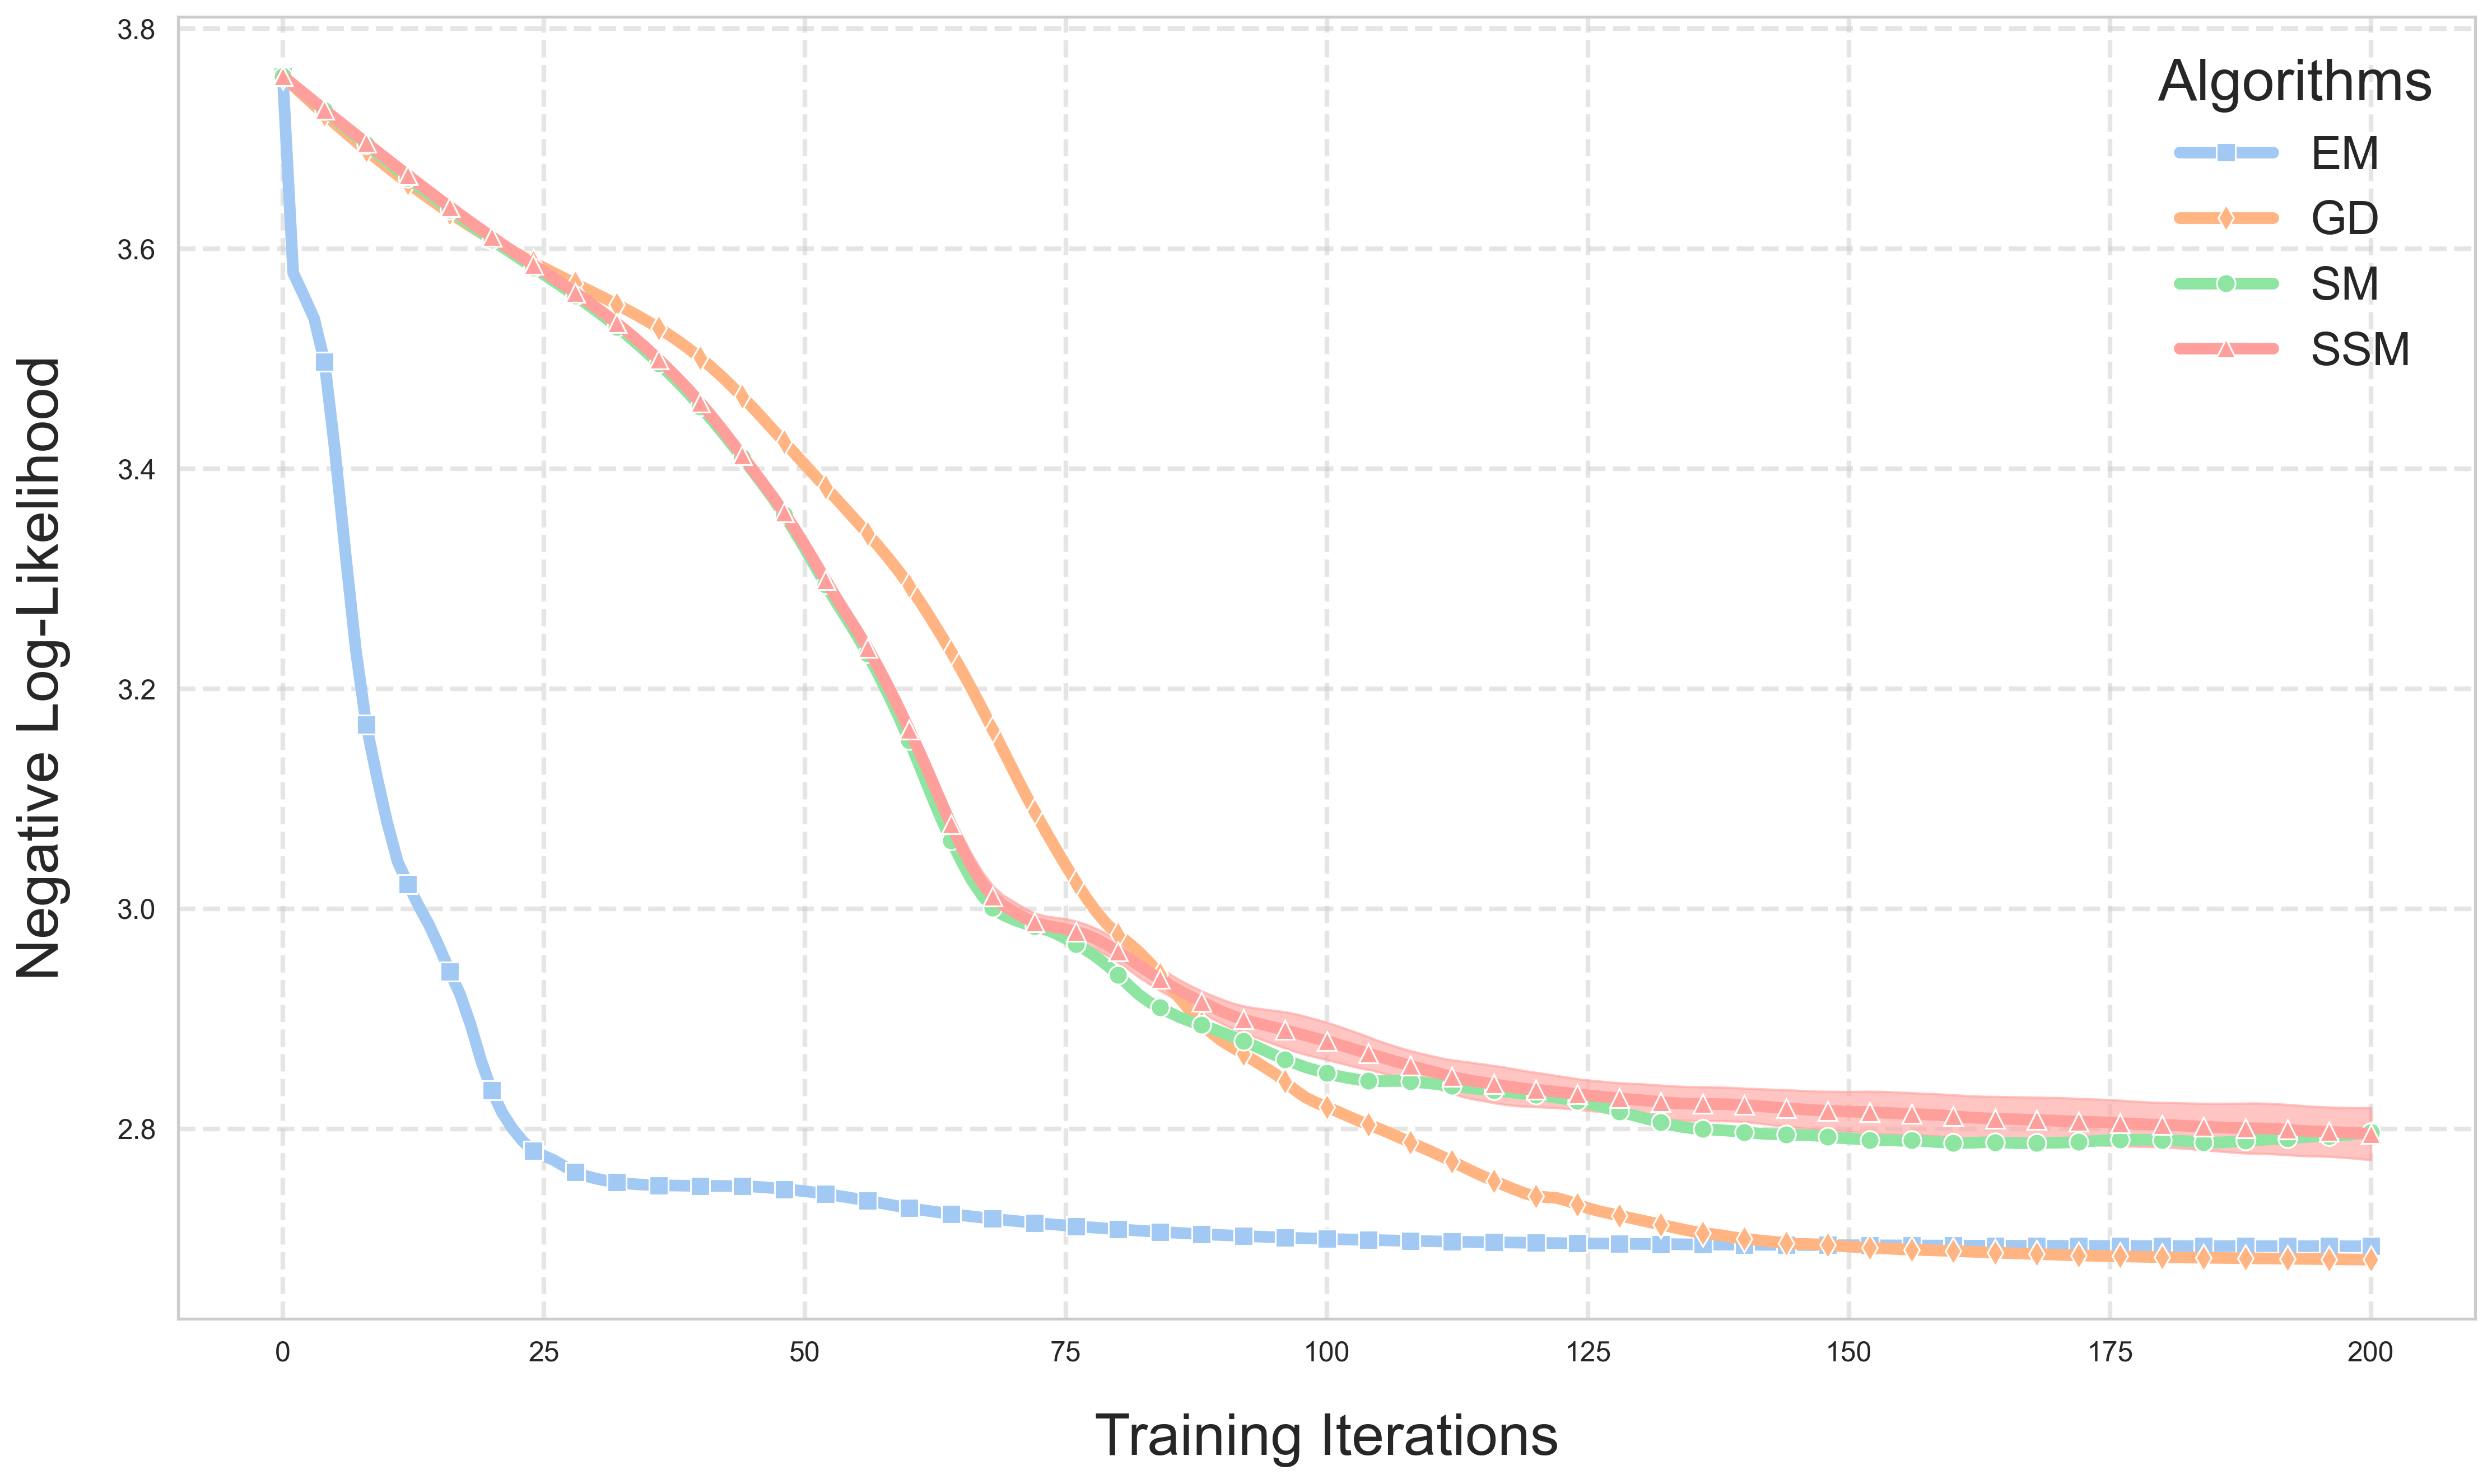
\includegraphics[width=0.8\textwidth]{figures/spirals/30_kmeans_logp.png}}
    \caption{Densities, Samples and NLL over Training Iterations}
\end{figure}

\begin{figure}[H]
    \centering
    \makebox[\textwidth][c]{\hspace{-0.4cm} 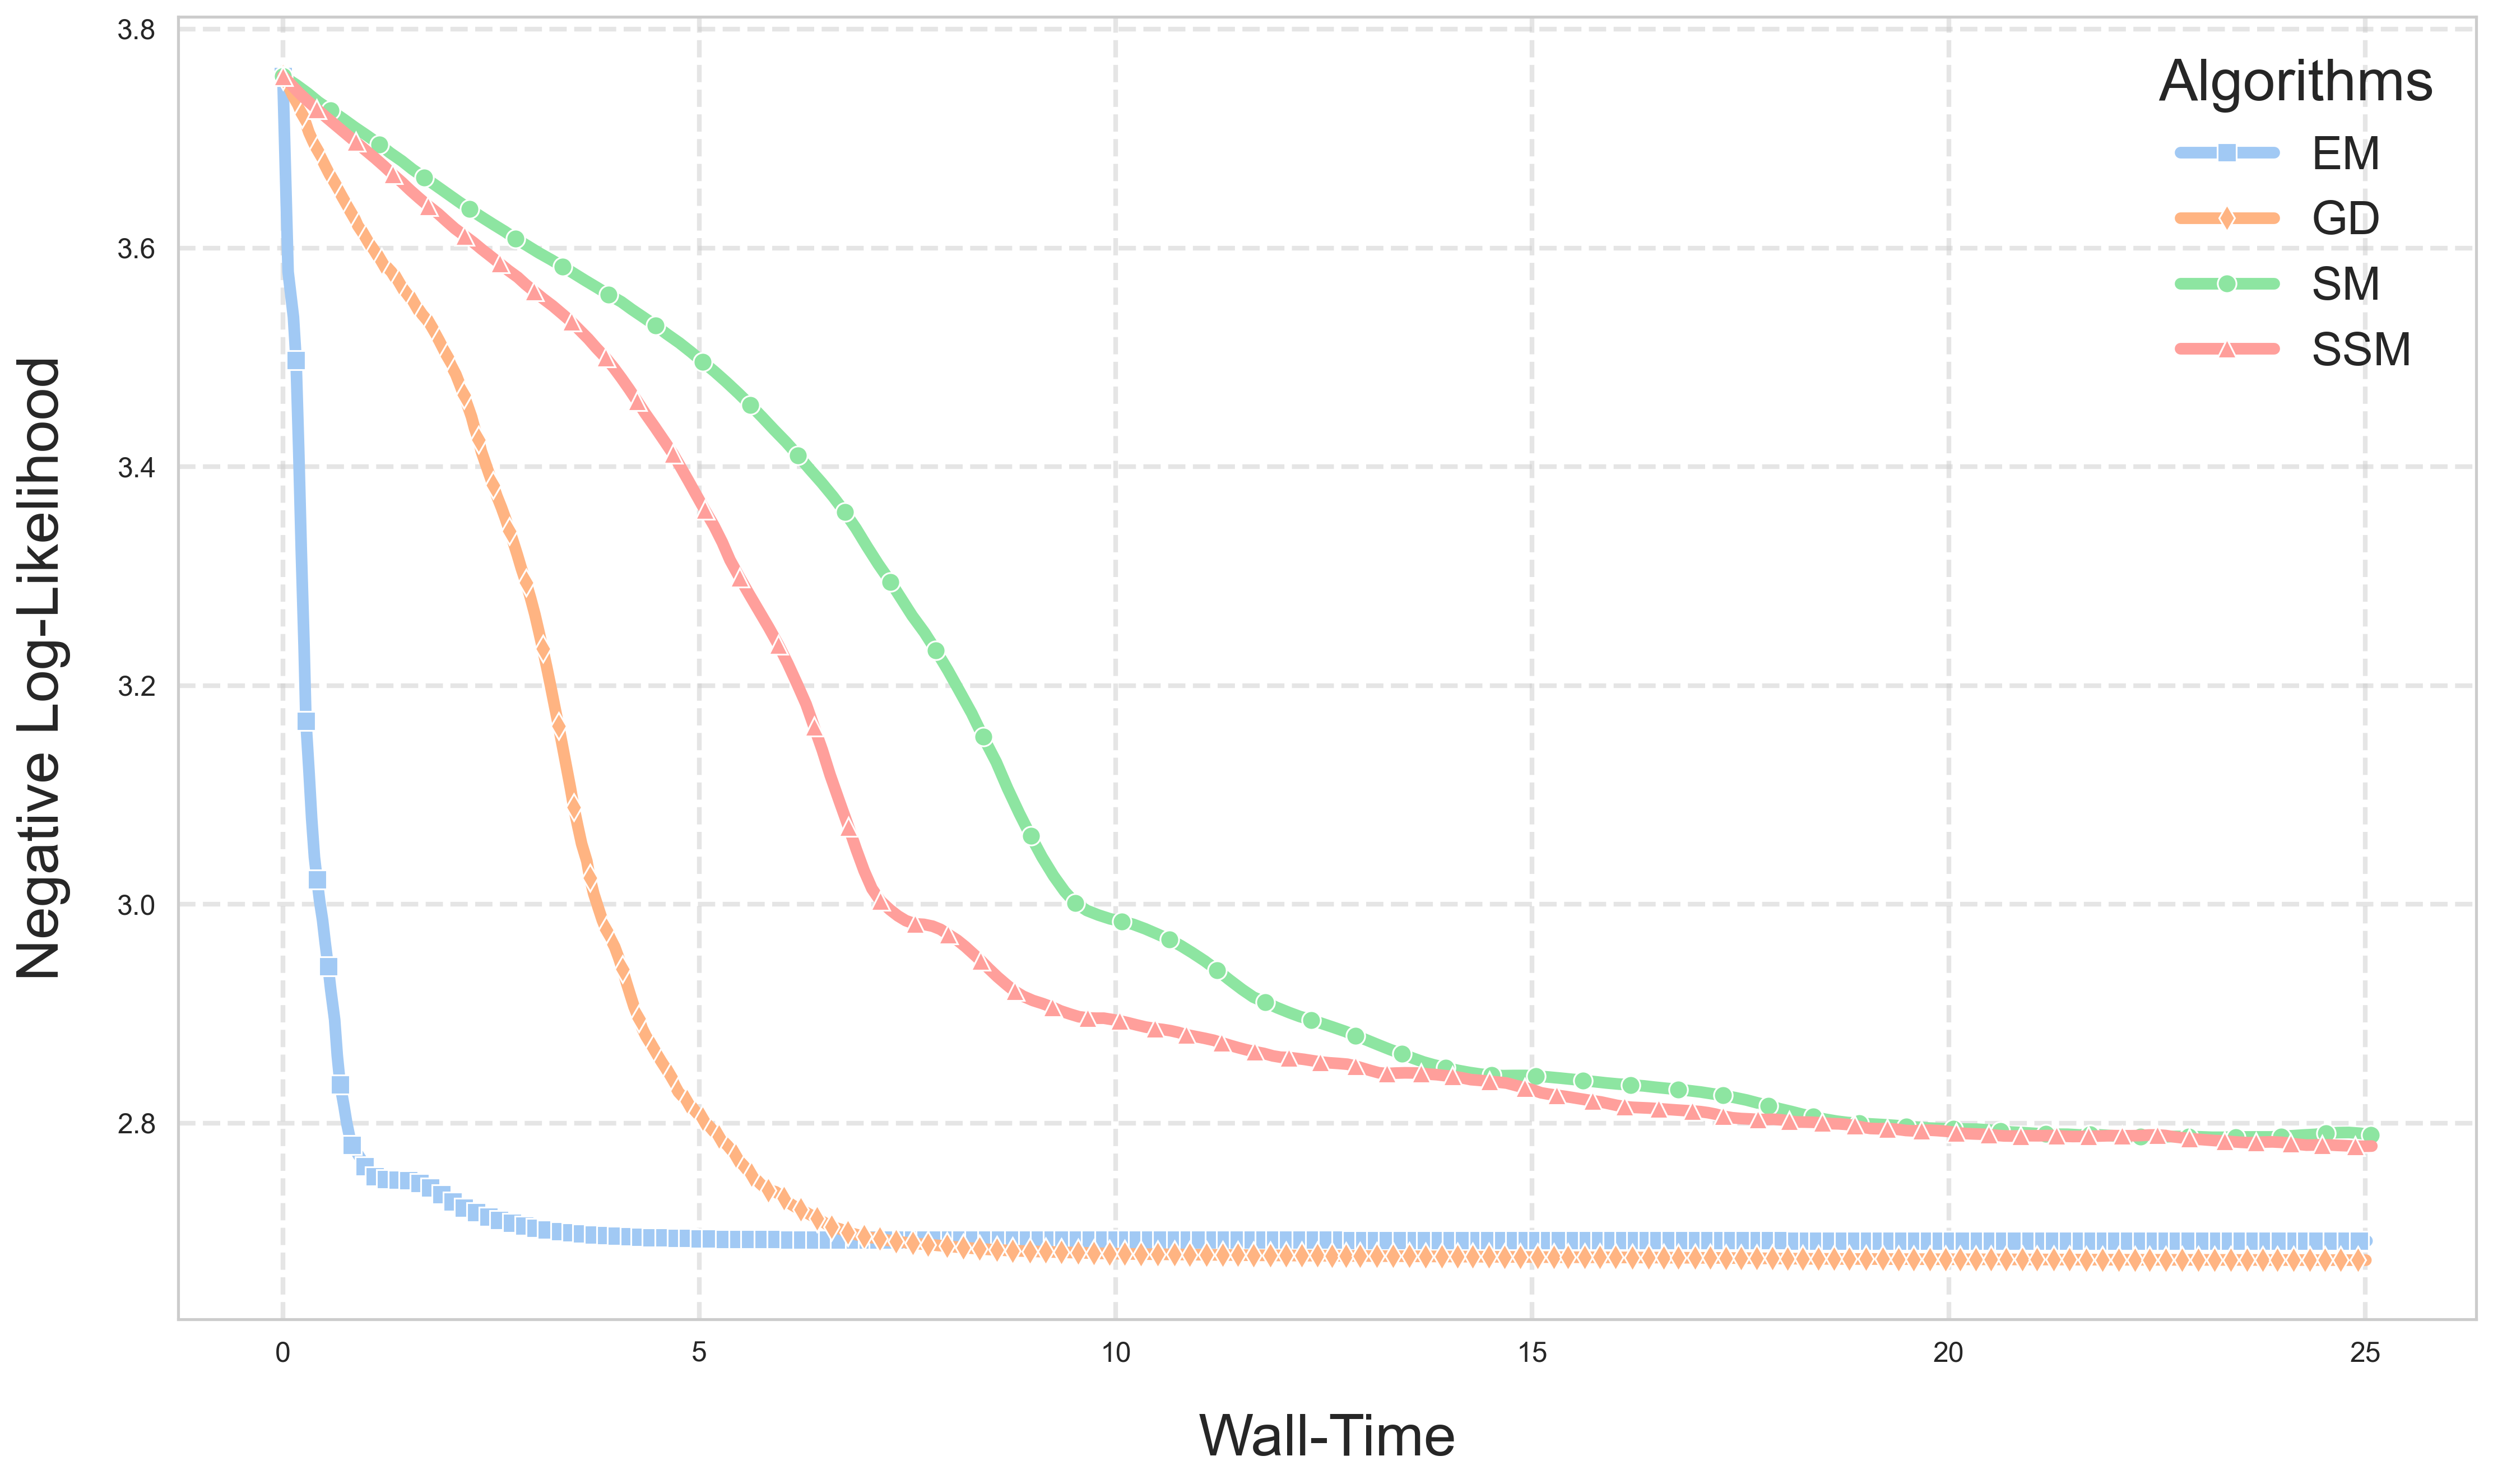
\includegraphics[width=0.8\textwidth]{figures/spirals/wall_time.png}}
    \caption{NLL over Time}
\end{figure}

\newpage
\begin{figure}[H]
    \centering
    \begin{subfigure}[b]{0.49\textwidth} 
        \centering
        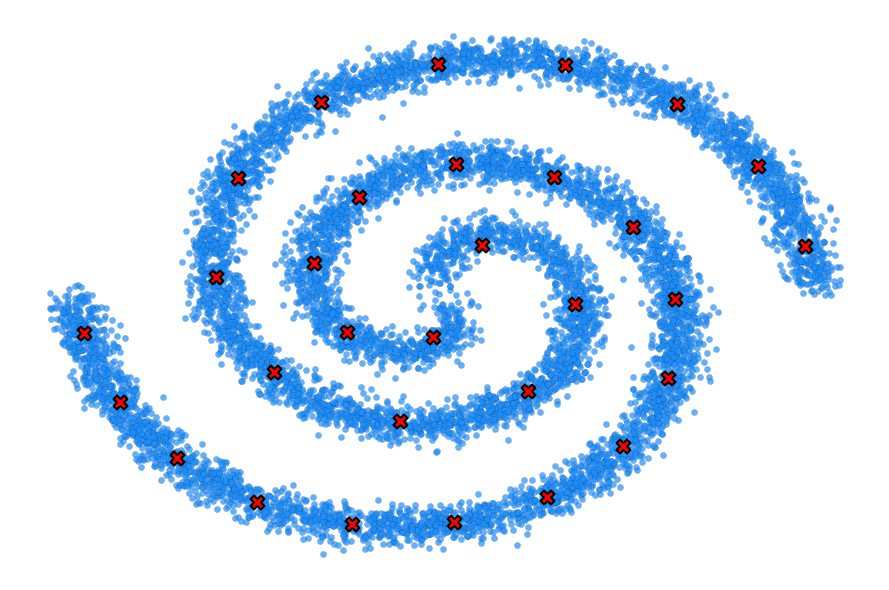
\includegraphics[width=\textwidth]{figures/spirals/30_kmeans_data.png}
        \caption{KMeans}
    \end{subfigure}
    \begin{subfigure}[b]{0.49\textwidth} 
        \centering
        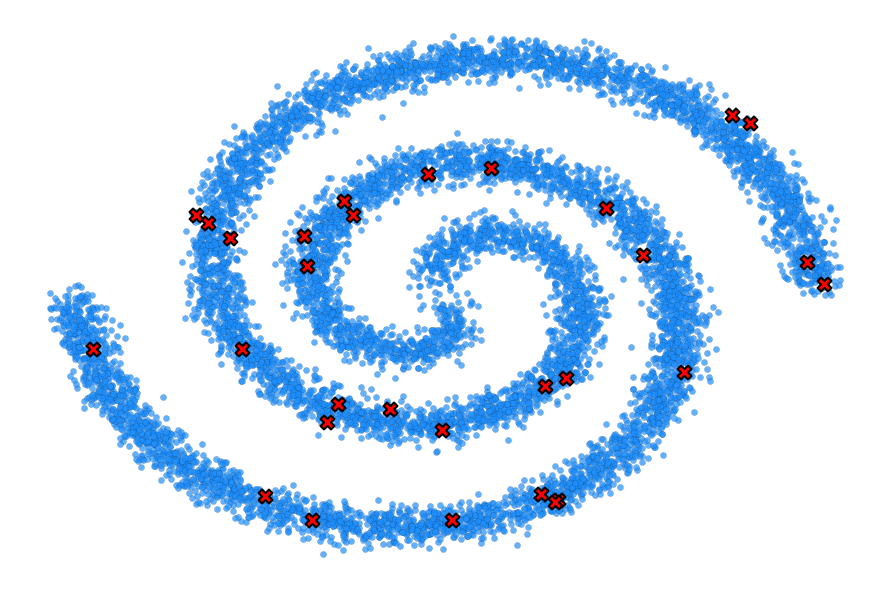
\includegraphics[width=\textwidth]{figures/spirals/30_random1_data.png} 
        \caption{Random}
    \end{subfigure} 
    \caption{KMeans vs. Random Initialization of means}
\end{figure}

\begin{figure}[H]
    \centering
    \makebox[\textwidth][c]{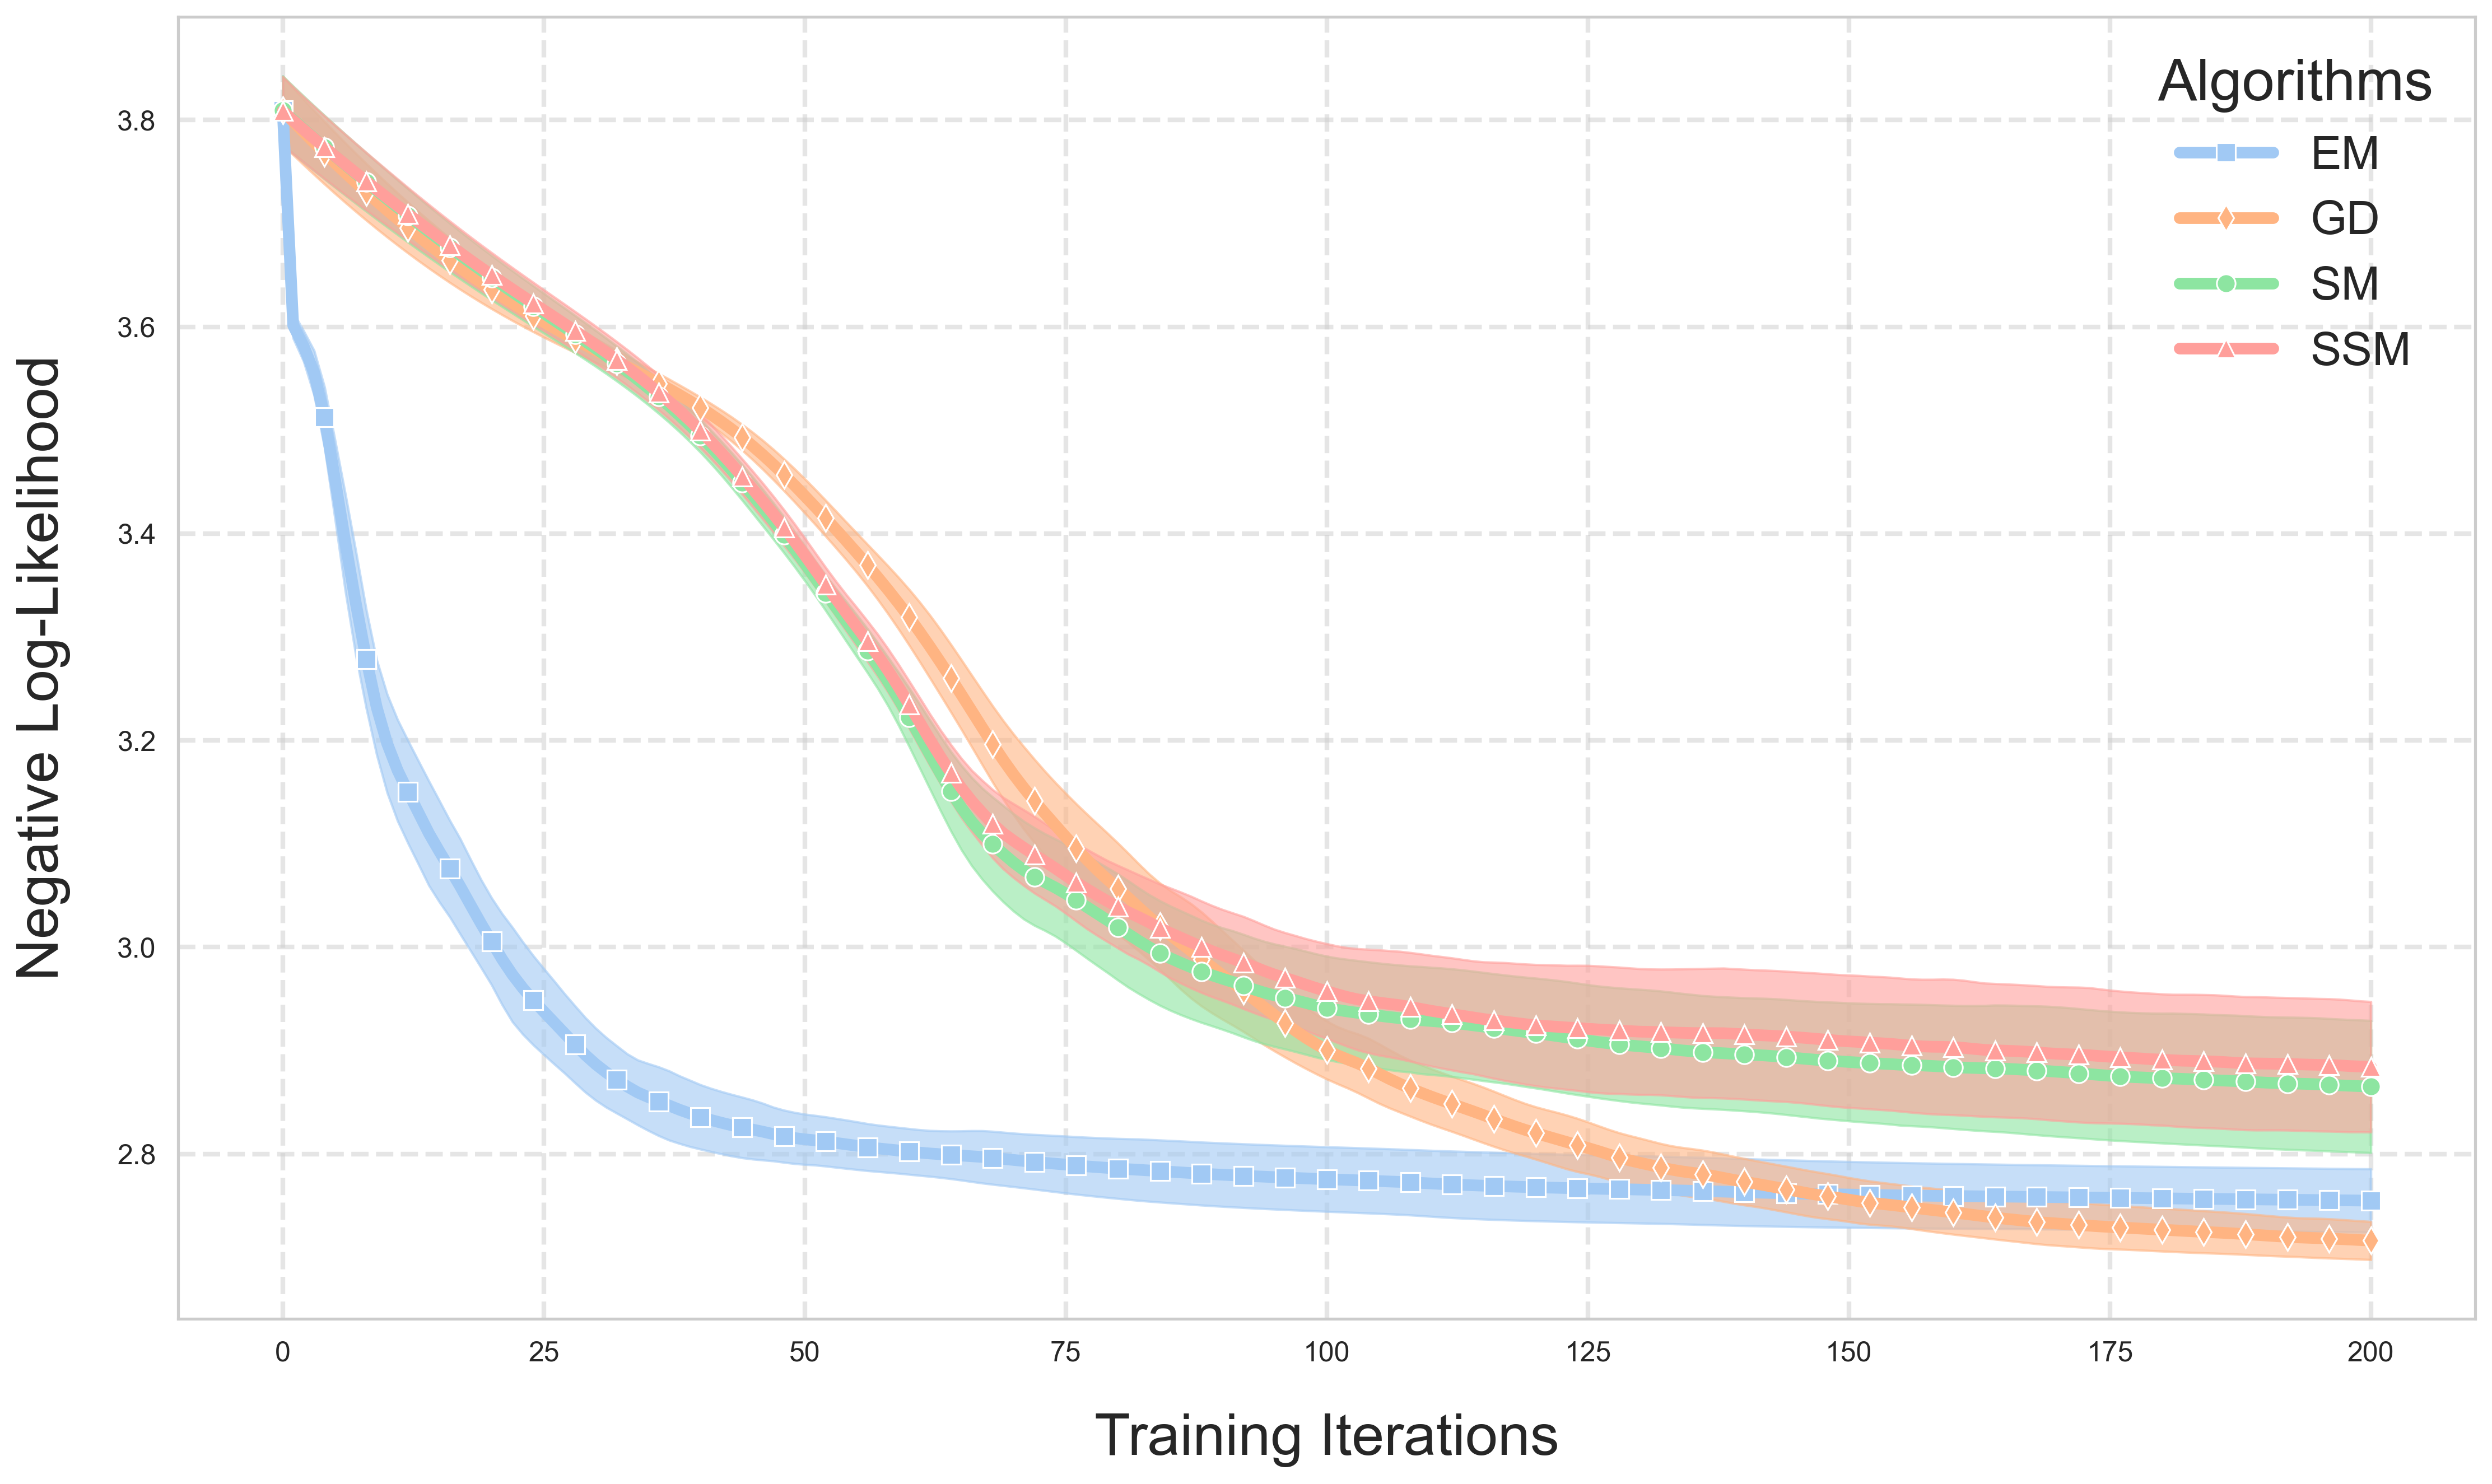
\includegraphics[width=0.9\textwidth]{figures/spirals/30_random_logp.png}}
    \caption{Negative Log Likelihood over Epochs with random parameter initialization}
\end{figure}

\begin{figure}[H]
    \centering
    \makebox[\textwidth][c]{\hspace*{-1cm} 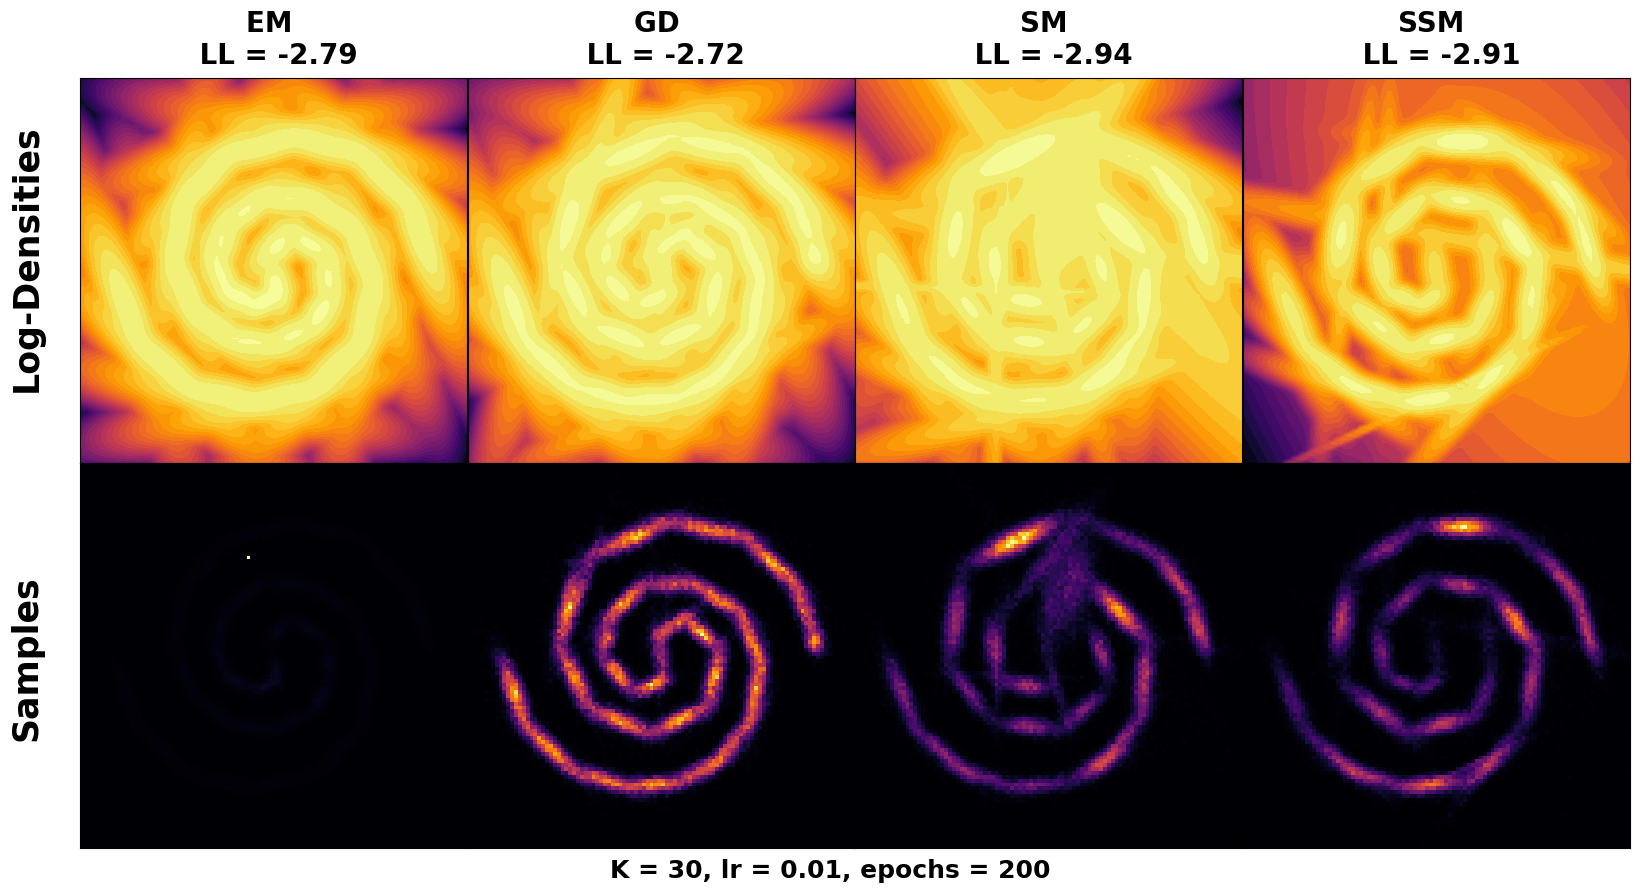
\includegraphics[width=0.8\textwidth]{figures/spirals/30_random1.png}}
    \vskip 5pt
    \makebox[\textwidth][c]{\hspace*{-1cm} 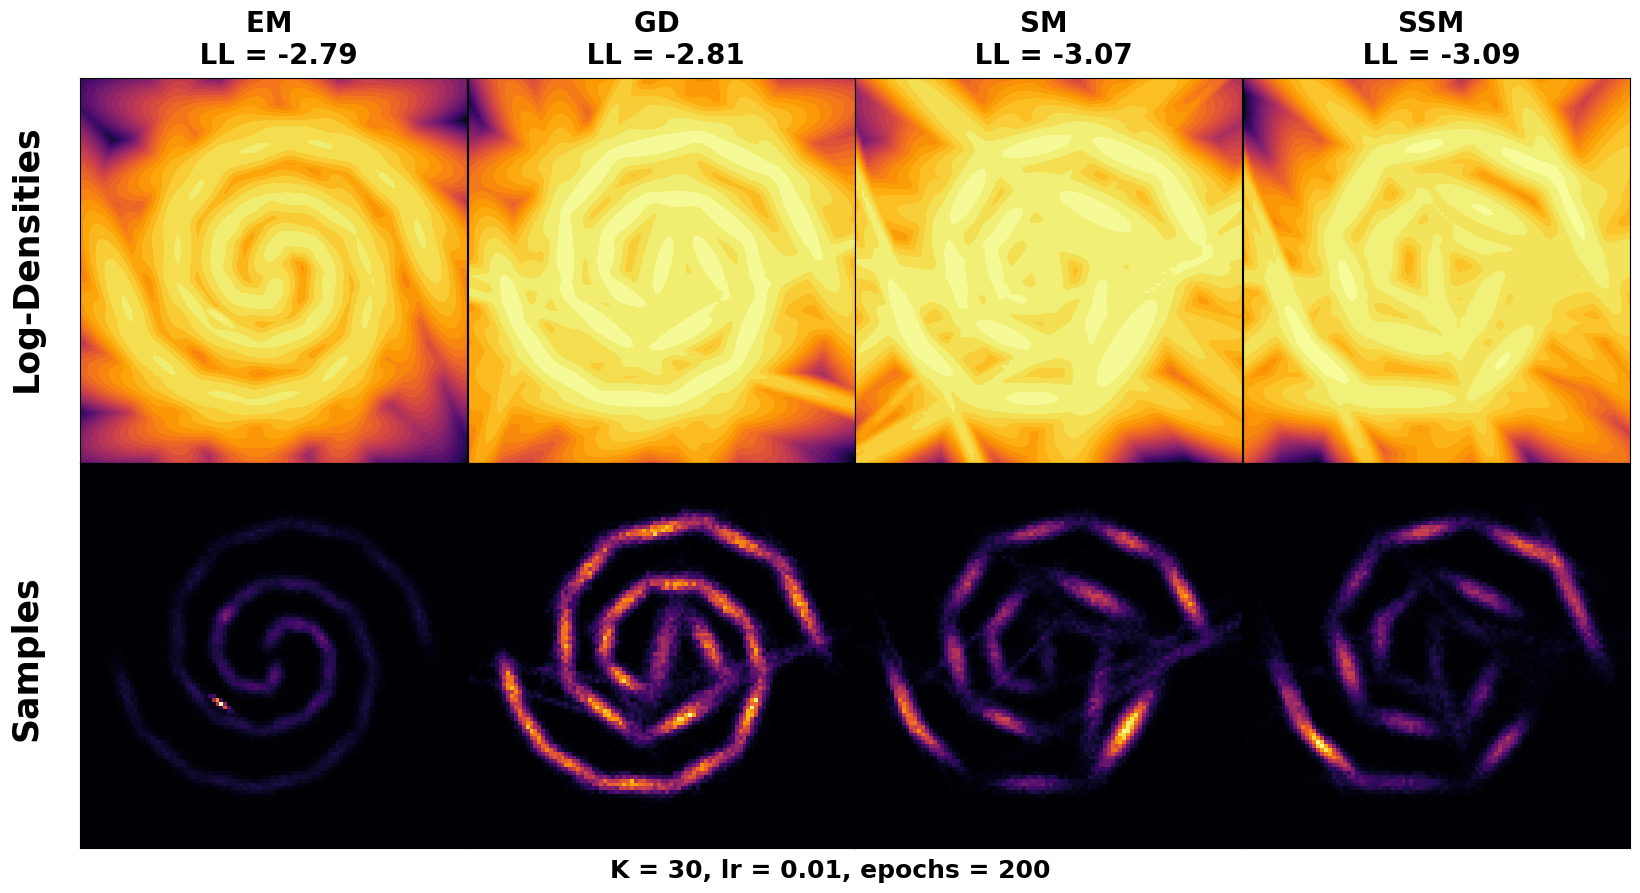
\includegraphics[width=0.8\textwidth]{figures/spirals/30_random2.png}}
    \vskip 5pt
    \makebox[\textwidth][c]{\hspace*{-1cm} 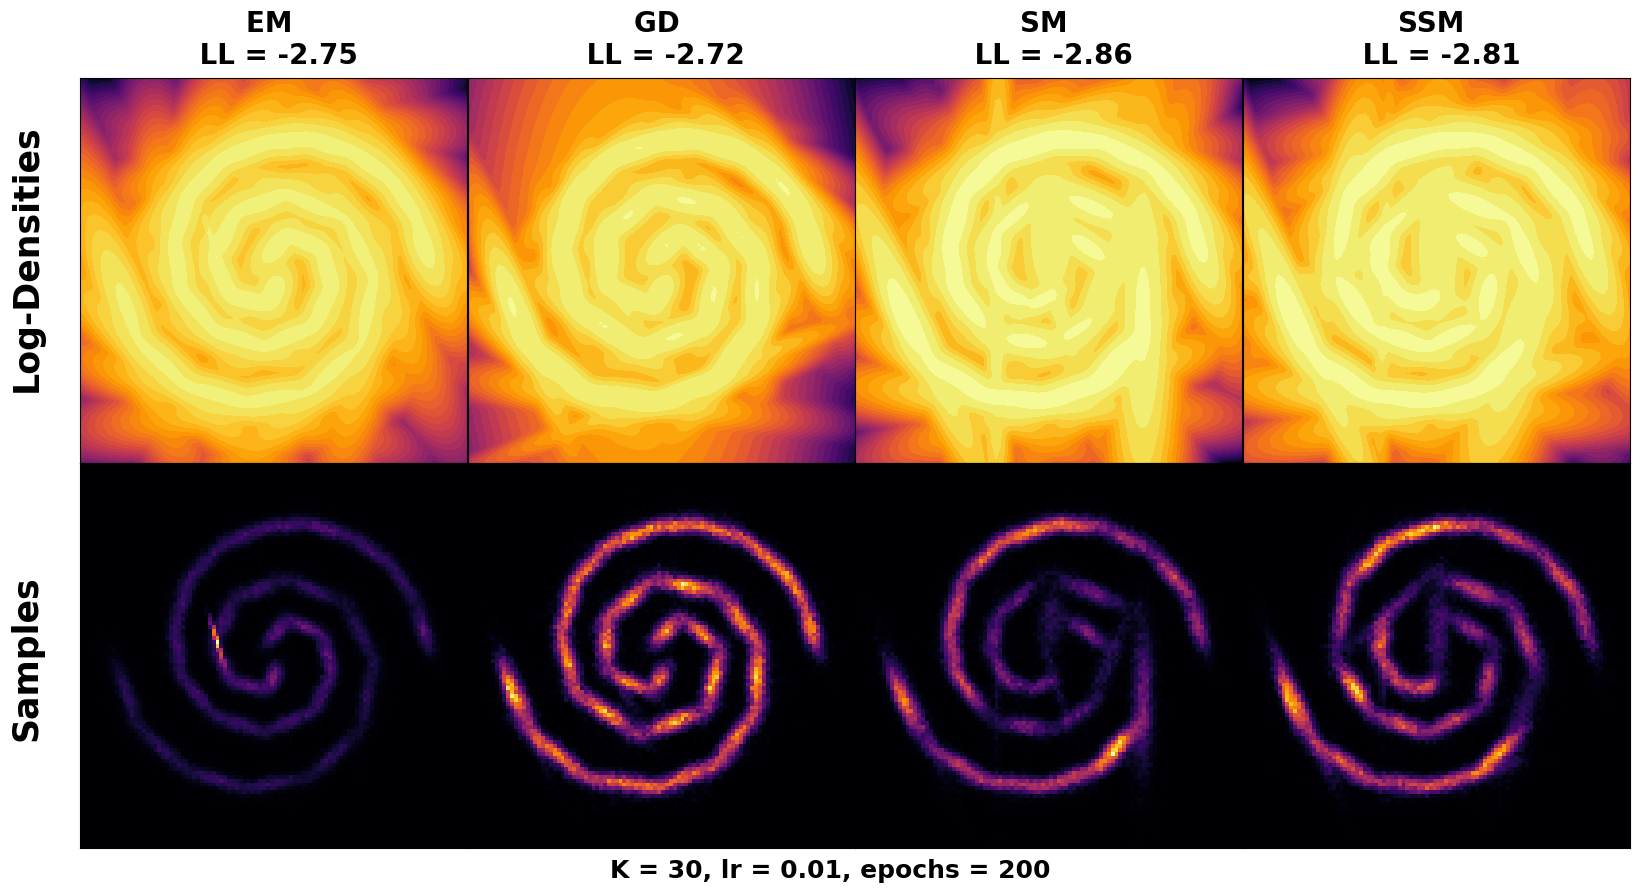
\includegraphics[width=0.8\textwidth]{figures/spirals/30_random3.png}}
    \caption{Densities and Samples for the spirals dataset}
\end{figure}

\subsubsection{Halfmoons Random Initialization Results}
\label{sec:app_halfmoons_rand}

\begin{figure}[H]
    \centering
    \makebox[\textwidth][c]{\hspace*{-1cm} 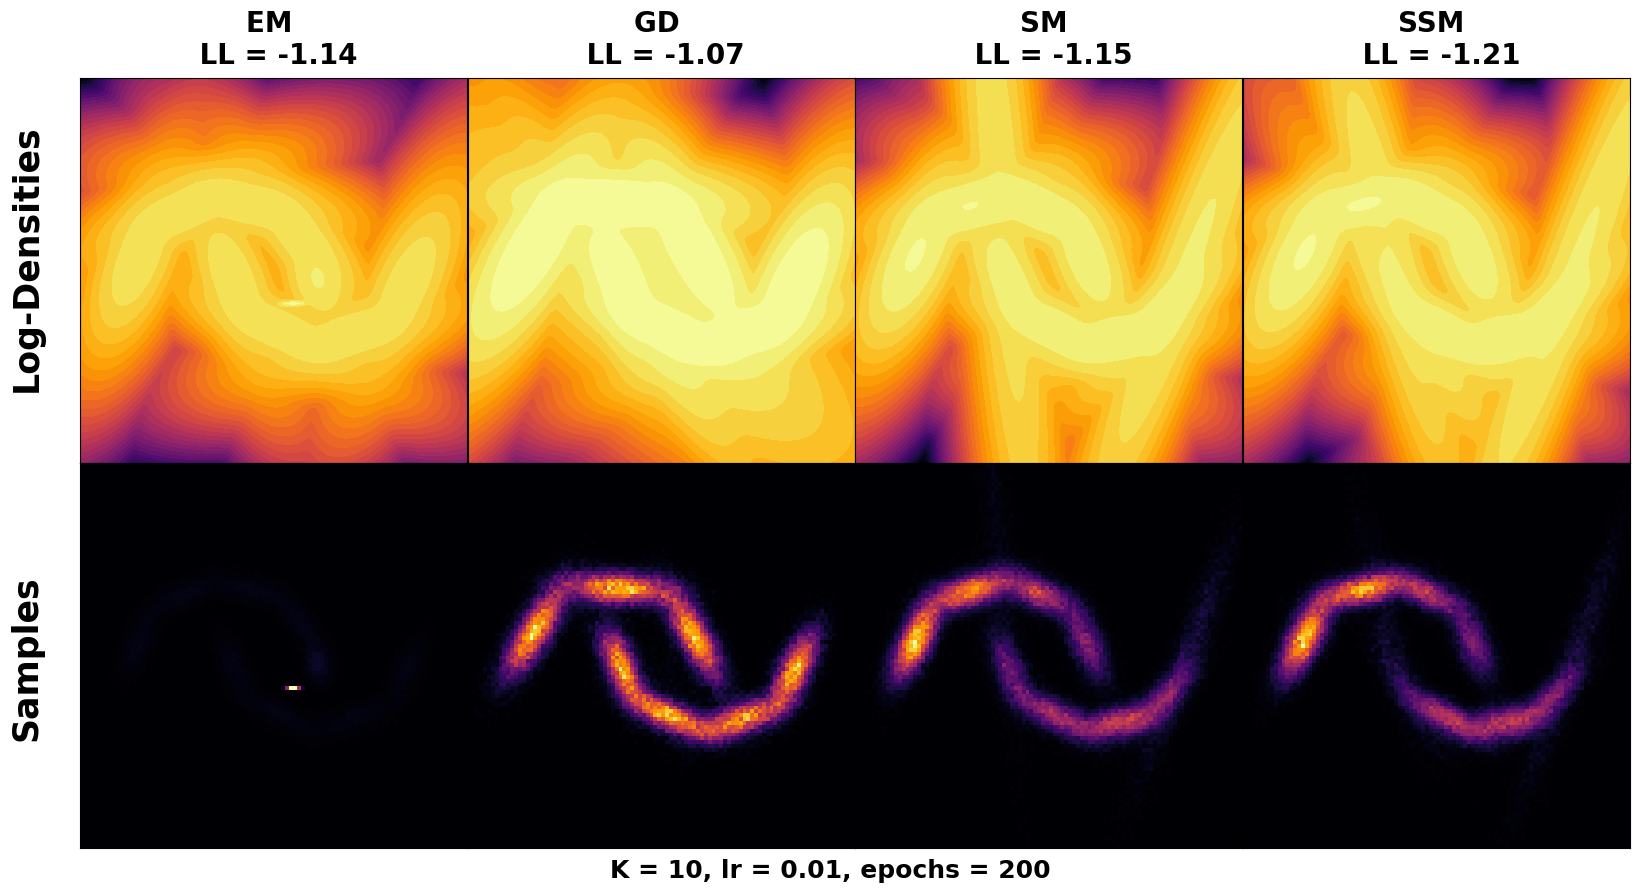
\includegraphics[width=0.8\textwidth]{figures/halfmoons/10_random1.png}}
    \vskip 5pt
    \makebox[\textwidth][c]{\hspace*{-1cm} 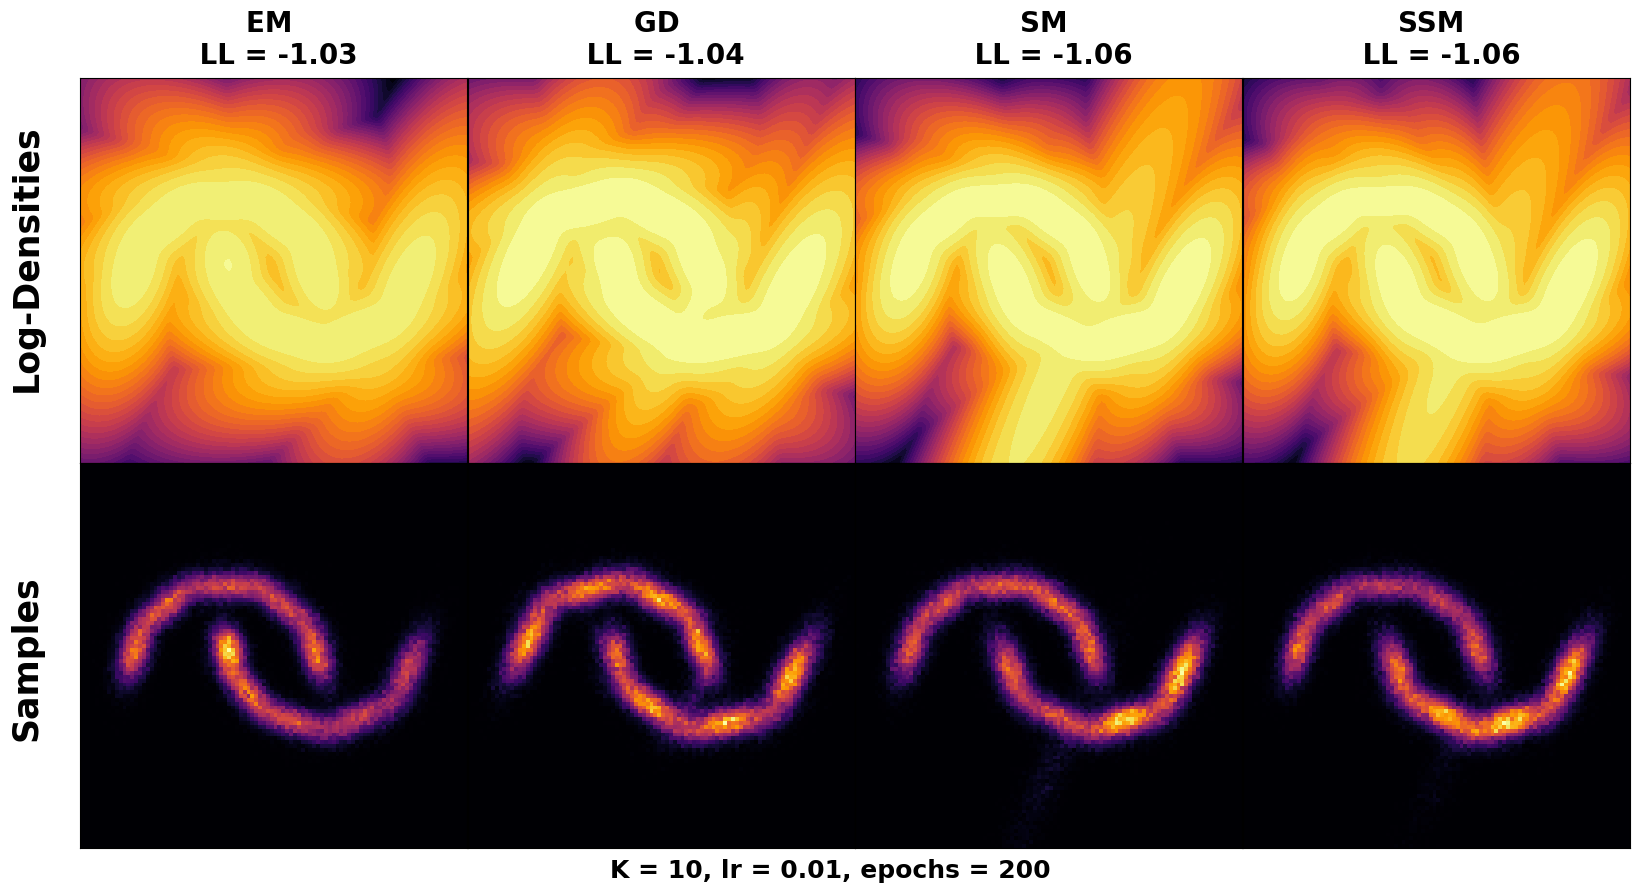
\includegraphics[width=0.8\textwidth]{figures/halfmoons/10_random2.png}}
    \vskip 5pt
    \makebox[\textwidth][c]{\hspace*{-1cm} 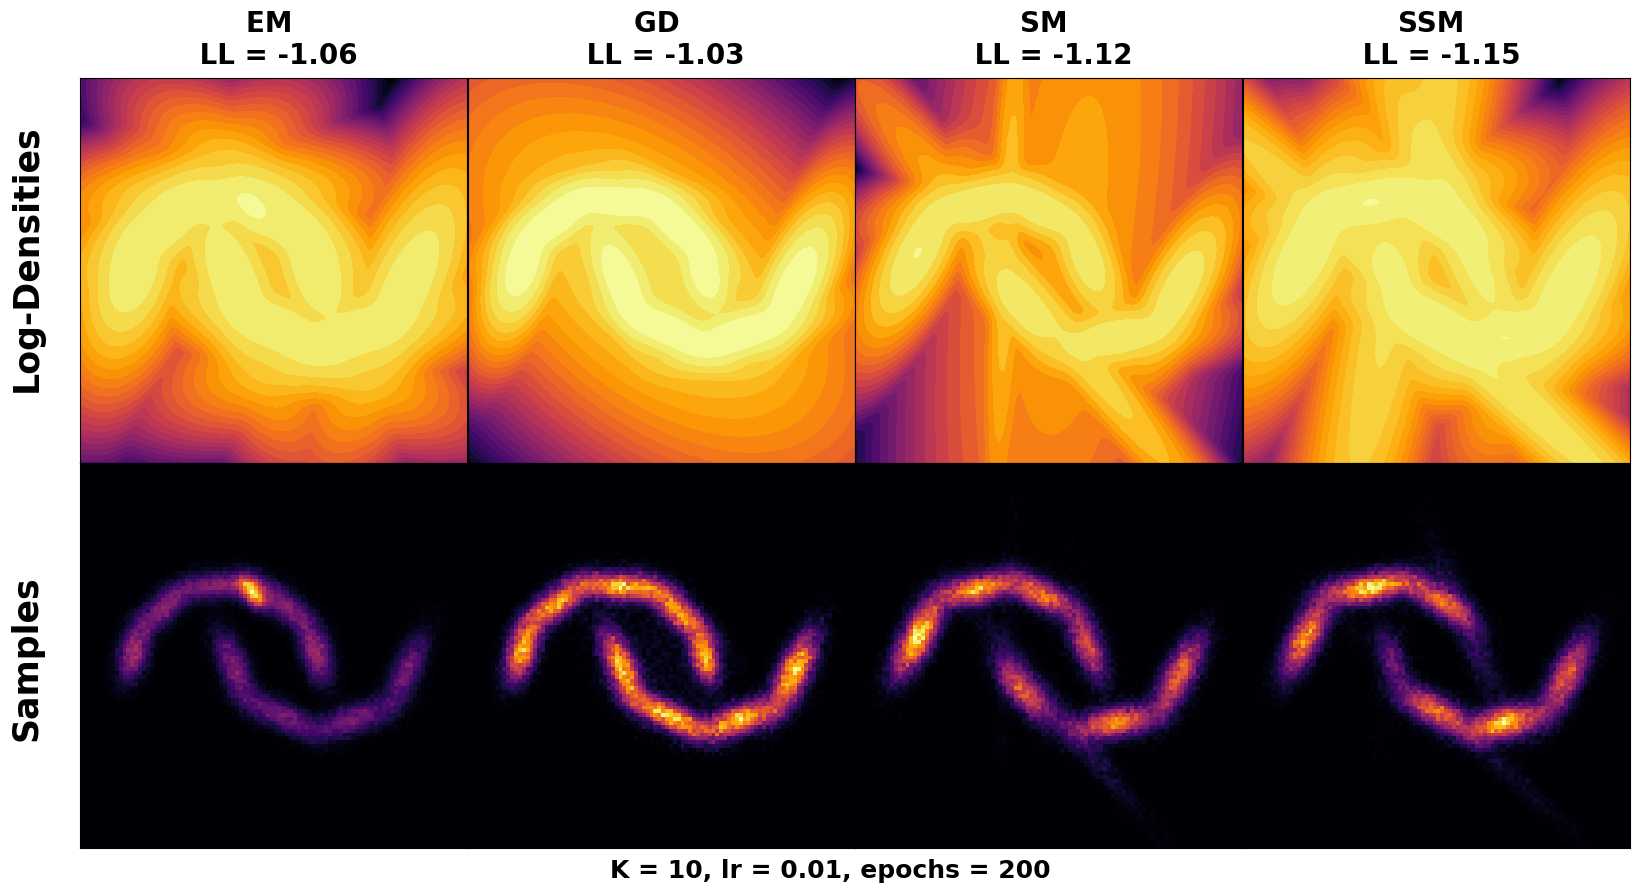
\includegraphics[width=0.8\textwidth]{figures/halfmoons/10_random3.png}}
    \caption{Densities and Samples for the halfmoon dataset}
\end{figure}

\subsubsection{FashionMNIST}
\label{sec:app_fashionmnist}

\begin{figure}[H]
    \centering
    \begin{subfigure}[b]{0.24\textwidth}
        \centering
        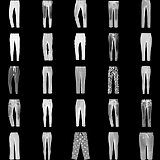
\includegraphics[width=\textwidth]{figures/einsum/fashion-mnist/1fashion-mnist_ground_truth.png}
        \caption{Ground Truth}
    \end{subfigure}
    \begin{subfigure}[b]{0.24\textwidth}
        \centering
        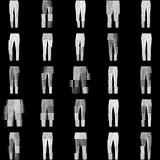
\includegraphics[width=\textwidth]{figures/einsum/fashion-mnist/1fashion-mnist_EM.png}
        \caption{EM (LL: -8230)}
    \end{subfigure}
    \begin{subfigure}[b]{0.24\textwidth}
        \centering
        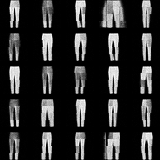
\includegraphics[width=\textwidth]{figures/einsum/fashion-mnist/1fashion-mnist_SGD.png} 
        \caption{SGD (LL: -8142)}
    \end{subfigure}
    \begin{subfigure}[b]{0.24\textwidth}
        \centering
        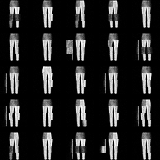
\includegraphics[width=\textwidth]{figures/einsum/fashion-mnist/1fashion-mnist_SSM.png}
        \caption{SSM (LL: -10797)}
    \end{subfigure}
    \caption{Samples and Log-Likelihood of FashionMNIST-class 1}
\end{figure}

\begin{figure}[H]
    \centering
    \begin{subfigure}[b]{0.24\textwidth}
        \centering
        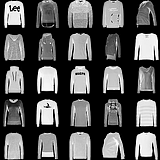
\includegraphics[width=\textwidth]{figures/einsum/fashion-mnist/2fashion-mnist_ground_truth.png}
        \caption{Ground Truth}
    \end{subfigure}
    \begin{subfigure}[b]{0.24\textwidth}
        \centering
        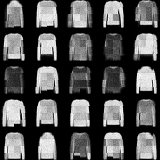
\includegraphics[width=\textwidth]{figures/einsum/fashion-mnist/2fashion-mnist_EM.png}
        \caption{EM (LL: -11973)}
    \end{subfigure}
    \begin{subfigure}[b]{0.24\textwidth}
        \centering
        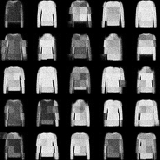
\includegraphics[width=\textwidth]{figures/einsum/fashion-mnist/2fashion-mnist_SGD.png} 
        \caption{SGD (LL: -12909)}
    \end{subfigure}
    \begin{subfigure}[b]{0.24\textwidth}
        \centering
        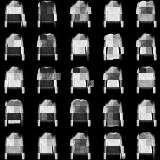
\includegraphics[width=\textwidth]{figures/einsum/fashion-mnist/2fashion-mnist_SSM.png}
        \caption{SSM (LL: -17594)}
    \end{subfigure}
    \caption{Samples and Log-Likelihood of FashionMNIST-class 2}
\end{figure}

\begin{figure}[H]
    \centering
    \begin{subfigure}[b]{0.24\textwidth}
        \centering
        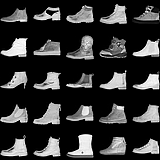
\includegraphics[width=\textwidth]{figures/einsum/fashion-mnist/9fashion-mnist_ground_truth.png}
        \caption{Ground Truth}
    \end{subfigure}
    \begin{subfigure}[b]{0.24\textwidth}
        \centering
        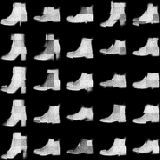
\includegraphics[width=\textwidth]{figures/einsum/fashion-mnist/9fashion-mnist_EM.png}
        \caption{EM (LL: -11173)}
    \end{subfigure}
    \begin{subfigure}[b]{0.24\textwidth}
        \centering
        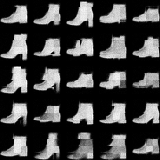
\includegraphics[width=\textwidth]{figures/einsum/fashion-mnist/9fashion-mnist_SGD.png} 
        \caption{SGD (LL: -11632)}
    \end{subfigure}
    \begin{subfigure}[b]{0.24\textwidth}
        \centering
        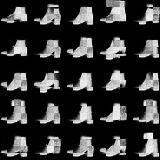
\includegraphics[width=\textwidth]{figures/einsum/fashion-mnist/9fashion-mnist_SSM.png}
        \caption{SSM (LL: -15864)}
    \end{subfigure}
    \caption{Samples and Log-Likelihood of FashionMNIST-class 9}
\end{figure}



